% !Mode:: "TeX:UTF-8"

\titlepage

\begin{frame}{说在前面}
	\linespread{1.5}
	  \begin{itemize}[<+-|alert@+>]
	    \item \ba{计算题请自行对答案}
% 	    \item 不记得自己哪周交作业
	  \end{itemize}
\end{frame}

% \begin{frame}{需要注意的问题}
% 	\linespread{1.5}
% 	  \begin{itemize}%[<+-|alert@+>]
% 	    \item L'Hospital法则
% 	    \begin{itemize}
% 	      \item \it 只能应用于“$\df{\bm{0}}{\bm{0}}$”
% 	      和“$\df{\bm{\infty}}{\bm{\infty}}$”型
% 	      \item \it 及时使用无穷小代换进行简化
% 	      \item \it 不正规的符号:\b 
% 	      $\xlongequal{\footnotesize\mbox{“L”}}$、
% 	      $\xlongrightarrow{\footnotesize\mbox{“L'Hospital法则”}}$、
% 	      $\df{\bm{0}}{\bm{0}}$、$\df{\bm{\infty}}{\bm{\infty}}$
% 	    \end{itemize}
% 	    \item Taylor公式
% 	    \begin{itemize}
% 	      \item \it Taylor多项式不包含余项
% 	      \item \it 合并同次幂的系数
% 	      \item \it 尽量按照幂次由低到高排列,最后写余项
% 	    \end{itemize}
% 	  \end{itemize}
% \end{frame}

\section{多元复合函数与隐函数的偏导数}

\begin{frame}
	\linespread{1.5}
	\ba{1.设$u=f\left(\df xy,\df yz\right)$,求$\df {\p u}{\p x},\df {\p u}{\p y}$
	和$\df {\p u}{\p z}$。}
	
	\bigskip
	
	\small 解:\it
	\begin{align*}
		u'_x&=f'_1\left(\df xy,\df yz\right)\df1y,\\
		u'_y&=-f'_1\left(\df xy,\df yz\right)\df x{y^2}
		+f'_2\left(\df xy,\df yz\right)\df1z,\\
		u'_x&=-f'_2\left(\df xy,\df yz\right)\df{y}{z^2}.
	\end{align*}
	\fin
\end{frame}

\begin{frame}
	\linespread{1.5}
	\ba{2.设$f(x,y)$一阶偏导连续,$f(1,1)=1,f\,'_x(1,1)=2$,
	$f\,'_y(1,1)=3$,又$\varphi(x)=f(x,f(x,x))$,求
	$\left.\df{\d\varphi^3(x)}{\d x}\right|_{x=1}$。}
	
	\bigskip
	
	\small 解:\it
	$$\varphi'(1)=f'_x(1,f(1,1))+f'_y(1,f(1,1))[f'_x(1,1)+f'_y(1,1)]
	=17,$$
	进而
	\begin{align*}
		\left.\df{\d\varphi^3(x)}{\d x}\right|_{x=1}
		&=\left.3\varphi^2(x)\varphi'(x)\right|_{x=1}=51.
	\end{align*}
	\fin
\end{frame}

\begin{frame}
	\linespread{1.5}
	\ba{3.设$z=xf\left(\df yx\right)+yg\left(x,\df xy\right)$,
	其中$f,g$均二次可微,求$\df{\p^2 z}{\p x\p y}$。}

	\bigskip
	
	\small 解:\it
	\begin{align*}
		z'_x&=f\left(\df yx\right)-f'\left(\df yx\right)\df{y}{x^2}
		+y\left[g'_1\left(x,\df xy\right)+g'_2\left(x,\df xy\right)\df1y\right],\\
		z''_{xy}&=f'\left(\df yx\right)\df1x
		-f''\left(\df yx\right)\df{y}{x^3}-f'\left(\df yx\right)\df1{x^2}\\
		&\quad+g'_1\left(x,\df xy\right)
		+g'_2\left(x,\df xy\right)\df1y\\
		&\quad y\left[-g''_{12}\left(x,\df xy\right)\df{x}{y^2}-g''_{22}\left(x,\df
		xy\right)\df{x}{y^3}-g'_2\left(x,\df xy\right)\df1{y^2}\right].
	\end{align*}
	\fin
\end{frame}

\begin{frame}
	\linespread{1.5}
	\ba{4.设$f(x,y)$一阶偏导数连续,且对任意实数$t$,有
	$f(tx,ty)=tf(x,y)$,
	证明:曲面$z=f(x,y)$上任一点$M$处的切平面与向径平行。}

	\bigskip
	
	\small 解:\it
	已知等式两边关于$t$求导,可得
	$$f'_1(tx,ty)x+f'_2(tx,ty)y=f(x,y),$$
	令$t=1$,整理后可得
	$$(f'_x(x,y),f'_y(x,y),-1)\cdot(x,y,f(x,y))=0,$$
	注意到$(f'_x(x,y),f'_y(x,y),-1)$为曲面上一点$(x,y,f(x,y))$处的法向量,从而
	可知曲面在该点处的切平面必与其该点的相近平行。\fin
\end{frame}

\begin{frame}
	\linespread{1.5}
	\ba{5.设$F(u,v)$具有一阶连续偏导数,且由$F\left(\df xz,\df yz\right)=0$
	可确定函数$z=z(x,y)$,求$x\df{\p z}{\p x}+y\df{\p z}{\p y}$。}

	\bigskip
	
	\small 解:\it
	对$F\left(\df xz,\df yz\right)=0$两边求微分,可得
	$$F'_1\left(\df xz,\df yz\right)\left(\df1z\d x-\df x{z^2}\d z\right)
	+F'_2\left(\df xz,\df yz\right)\left(\df1z\d y
	-\df{y}{z^2}\d z\right)=0,$$
	由此可得
	$$
	z'_x=\df{zF'_1}{xF'_1+yF'_2},\quad
	z'_y=\df{zF'_2}{xF'_1+yF'_2},
	$$
	进而可得
	$$x\df{\p z}{\p x}+y\df{\p z}{\p y}=z.$$\fin
\end{frame}

\begin{frame}
	\linespread{1.5}
	\ba{6.设$y=f(x,t)$,其中$t$是由$F(x,y,t)=0$所确定的隐函数,$f,F$具有
	一阶连续偏导数,求$\df{\d y}{\d x}$。}

	\bigskip
	
	\small 解:\it
	在$y=f(x,t)$和$F(x,y,t)=0$两边同时求微分,可得
	$$
		\left\{\begin{array}{l}
			\d y=f'_1\d x+f'_2\d t,\\
			F'_1\d x+F'_2\d y+F'_3\d t=0.
		\end{array}\right.
	$$
	消去$\d t$,整理后可得
	$$\df{\d y}{\d x}=\df{f'_2F'_1+f'_1F'_3}{F'_3-f'_2F'_2}.$$\fin
	
	\ba{注:利用微分运算计算偏导数,在计算过程中可以不必考虑哪些变量时自变量,
	哪些是因变量,而将该问题留到最后决定即可。}
\end{frame}

\begin{frame}
	\linespread{1.5}
	\ba{7.设$u=u(x,y),x=r\cos\theta,y=r\sin\theta$,将方程
	$x\df{\p u}{\p y}-y\df{\p u}{\p x}=0$
	化为$u$关于$r,\theta$的偏导数的方程。}
	
	\small 解:\it
	由已知$r=\sqrt{x^2+y^2},\theta=\arctan\df yx$,从而
	$$
		r'_x=\df xr,\quad r'_y= \df yr,\quad
		\theta'_x=-\df y{r^2},\quad \theta'_y=\df x{r^2}. 
	$$
	从而
	\begin{align*}
		u'_x&=u'_rr'_x+u'_{\theta}\theta'_x=\df{u'_rxr-u'_{\theta}y}{r^2},\\
		u'_y&=u'_rr'_y+u'_{\theta}\theta'_y=\df{u'_ryr+u'_{\theta}x}{r^2}.
	\end{align*}
	于是
	$$x\df{\p u}{\p y}-y\df{\p u}{\p x}=u'_{\theta},$$
	进而可知原方程可化为$u'_{\theta}=0$。\fin
\end{frame}

\section{方向导数、梯度、Hessian矩阵与多元Taylor公式}

\begin{frame}
	\linespread{1.5}
	\ba{1.求曲面$z=x^2+y^2$上的点$(1,1,2)$处沿椭圆$\df{x^2}{8}+\df{y^2}{2}=1$
	在$(2,1)$的外法向的方向导数。}
	\pause

% 	\bigskip
	\small 证:\it
	由梯度的几何意义,椭圆$\df{x^2}{8}+\df{y^2}{2}=1$在$(2,1)$的外法向为
	$\bm{u}=\left(\df12,1\right)$。从而所求方向导数
	$$D_uz(1,1,2)=\bm{e}_u\cdot\bigtriangledown z(1,1)
	=\left(\df1{\sqrt5},\df2{\sqrt5}\right)\cdot (2,2)=\df6{\sqrt5}.$$
	\fin
	
	\ba{注:将椭圆视为曲面$z=\df{x^2}{8}+\df{y^2}{2}$的等值线,再由$z$增大的方向
	是向外的,可确定梯度的方向即为椭圆的外法向。}
\end{frame}

\begin{frame}
	\linespread{1.5}
	\ba{2.试证曲面$\sqrt{x}+\sqrt y+\sqrt z=\sqrt a\,(a>0)$
	在任一点处的切平面在三个坐标轴上的截距之和为常数。}
	
	\small 解:\it 任取曲面上一点$(x_0,y_0,z_0)$,则曲面该点处的法向量为
	$$\bm{n}=\left(\df1{\sqrt{x_0}},\df1{\sqrt{y_0}},
	\df1{\sqrt{z_0}}\right),$$
	从而切平面为
	$$\df1{\sqrt{x_0}}(x-x_0)+\df1{\sqrt{y_0}}(y-y_0)
	+\df1{\sqrt{z_0}}(z-z_0)=0,$$
	其在三个坐标轴上的截距分别为$a\sqrt{x_0},a\sqrt{y_0},a\sqrt{z_0}$,
	由此易知结论成立。\fin
\end{frame}

\begin{frame}
	\linespread{1.5}
	\ba{3.已知曲面方程$z=xe^{y/x}$,证明:曲面上任一点$M$处的法线与其
	向径垂直。}
	
	\bs
	
	\small 证:\it 曲面上任一点$(x,y,z)$处的法向量为
	$$\bm{n}=\left(e^{y/x}\left(1-\frac yx\right),e^{y/x},-1\right),$$
	向径为$\bm{r}=(x,y,z)$,容易验证$\bm{n}\cdot\bm{r}=0$。\fin
\end{frame}

\begin{frame}
	\linespread{1.5}
	\ba{4.求函数$xe^{x+y}$在原点处带Peano余项的二阶Taylor公式。}
	\pause

% 	\bigskip
	\small 解:\it 注意到
	$$e^x=1+x+\circ(x),$$
	故易知
	$$e^{x+y}=1+x+y+\circ(\sqrt{x^2+y^2}),$$
	进而可知
	$$xe^{x+y}=x+x^2+xy+\circ(x^2+y^2).$$
	\fin
\end{frame}

\section{多元函数的极值与条件极值}

\begin{frame}
	\linespread{1.5}
	\ba{1.求内接于椭球面$\df{x^2}{a^2}+\df{y^2}{b^2}+\df{z^2}{c^2}=1$
	的长方体的最大体积。}
	\pause

% 	\bigskip
	\small 解:\it 设$(x,y,z)$为第一卦限内的椭球面上任一点,则以之为顶点的长方体体积为
	$V=8xyz$。由平均值不等式,
	$$\sqrt[3]{\df{x^2y^2z^2}{a^2b^2c^2}}
	\leq\df13\left(\df{x^2}{a^2}+\df{y^2}{b^2}+\df{z^2}{c^2}\right)=\df13,$$
	且当$\df{x^2}{a^2}=\df{y^2}{b^2}=\df{z^2}{c^2}$时取等号,从而可知
	$V\leq\df{(abc)^{\frac32}}{3\sqrt3}$,
	也即椭球的最大内接长方体体积为$\df{(abc)^{\frac32}}{3\sqrt3}$,此时
	$x=\df{a}{\sqrt3},y=\df{b}{\sqrt3},z=\df{c}{\sqrt3}$。\fin
\end{frame}

\begin{frame}
	\linespread{1.5}
	\ba{2.某公司的产品广告有电台和报纸两种发布途径,经研究发现,产品销售收入$U$(万元)与
	  投入的电台广告费用$T$(万元)和投入的报纸广告费用$P$(万元)满足
	  $$U=15+14T+32P-8TP-2T^2-10P^2.$$
	  \vspace{-3ex}
	  \begin{enumerate}[(1)]
	    \item 在广告预算不封顶的情况下,求公司的最优广告策略;
	    \item 若广告总预算上限为$1.5$万元,求公司的最优广告策略。
	  \end{enumerate}}
\end{frame}

\begin{frame}
	\linespread{1.5}
	
	\small 解:(1)\it 由已知可得
	$$\bigtriangledown U=(14-8P-4T,32-8T-20P),$$
	令$\bigtriangledown U=0$,可解得$P=1,T=1.5$。又
	$$\bigtriangledown^2U=\left[\begin{array}{cc}
		-4 & -8 \\ -8 & -20
	\end{array}\right]$$
	是负定的,故可知此时公司的最优广告策略为电视广告投入$1$万元,
	报纸广告投入$1.5$万元。
\end{frame}

\begin{frame}
	\linespread{1.4}
	
	\small (2)\it 注意到驻点$(1,1.5)$不超出了预算上限,故此时只需考虑取值区域
	$$0\leq T\leq T+P\leq 1.5$$
	边界上的极值问题。
	
	当$T=0,0\leq P\leq 1.5$时,$U=15+32P-10P^2$,
	易得其最大值为$40.5$,对应地$P=1.5$;
	
	当$P=0,0\leq T\leq 1.5$时,$U=15+14T-2T^2$,易得其最大值为
	$31.5$,对应地$T=1.5$;
	
	当$0\leq T\leq T+P=1.5$时,$U=4(10.125-T^2)$,易得其最大值为
	$40.5$,此时$T=0,P=1.5$。
	
	综上可知,在广告预算上限为$1.5$万元时,最佳的广告投入策略是
	全部投入报纸广告。\fin
\end{frame}

\begin{frame}
	\linespread{1.5}
	\ba{3.已知$\lim\limits_{(x,y)\to(0,0)}\df{f(x,y)-4xy}{x^2+y^2}=1$,
	判断$(0,0)$是否为$f(x,y)$的极值点,若是,是极大值还是极小值?}
	\pause

% 	\bigskip
	\small 解:\it 由已知可得
	$$f(x,y)=4xy+x^2+y^2+\circ(x^2+y^2),$$
	进而可知
	$$\bigtriangledown f(0,0)=(0,0),\quad
	\bigtriangledown^2f(0,0)=\left[\begin{array}{cc}
		2 & 4 \\ 4 & 2
	\end{array}\right],$$
	由此易知原点为$f(x,y)$的鞍点。\fin
\end{frame}

% \begin{frame}{出现的问题}
% 	\linespread{1.5}
% 	  \begin{itemize}%[<+-|alert@+>]
% 	    \item 作业进度慢!
% 	    \item 概念问题
% 	    \begin{itemize}
% 	      \item \b\it 幂级数展开不熟练
% 	      \item \b\it Maclaurin级数和关于$(x-x_0)$的幂级数分不清
% 	    \end{itemize}
% 	    \item 过程不规范或不完整
% 	    \begin{itemize}
% 	      \item \b\it 求收敛域要单独讨论端点的敛散性
% 	      \item \b\it 相同幂次的项要合并,并按幂次从小到大排列
% 	      \item \b\it 书写潦草随意\pause
% 	    \end{itemize}
% 	    \item \ba{雷同!!!}
% 	  \end{itemize}
% \end{frame}

% \begin{frame}
% 	\linespread{1.5}
% 	\ba{3.设$D$是由曲线$y=\sin x+1$与三条直线$x=0,x=\pi,y=0$
% 	所围成的曲边梯形,求$D$绕$x$轴旋转一周所围成的旋转体的体积。
% 	}
% 	\pause
% 	
% % 	\bigskip
% 	
% 	\begin{columns}
% 		\begin{column}{.5\textwidth}
% 			\begin{center}
% 				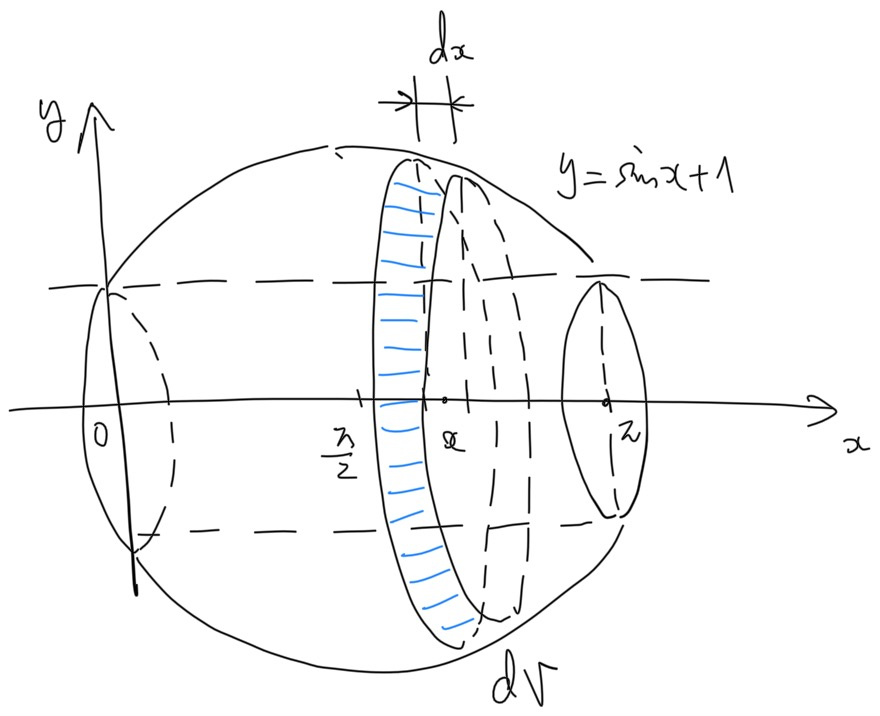
\includegraphics[width=.9\textwidth]{./images/ch6/sinx1cs.jpg}
% 		% 		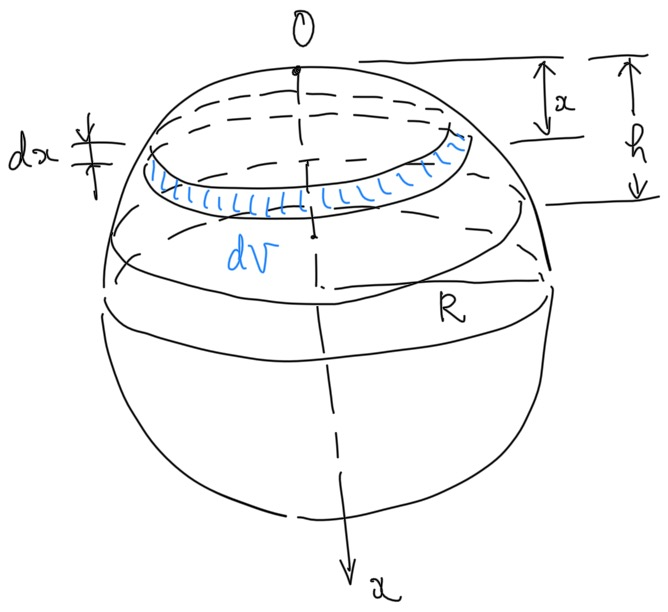
\includegraphics[width=6cm]{./images/ch6/topSp.jpg}
% 			\end{center}		
% 		\end{column}
% 		\begin{column}{.5\textwidth}
% 			\small 解:\it
% 			如图,体积微元$\d V=\pi y^2\d x$,	故所求体积
% 			$$
% 				V=\dint_0^{\pi}\pi(\sin x+1)^2\d x=\df32\pi^2.
% 			$$
% 		\end{column}
% 	\end{columns}
% \end{frame}